\documentclass[../main.tex]{subfiles}
\graphicspath{{\subfix{../images/}}}

\begin{document}

\hypertarget{attack-surface-approximation-module}{%
\chapter{The Attack Surface Approximation
Module}\label{attack-surface-approximation-module}}

Aside from the internal procedures that are automated, the software
should have ways of interacting with the outside world, either the
environment or the users. The following are the most commonly utilized
communication channels:

\begin{itemize}
\tightlist
\item
  \texttt{stdin} (standard input);
\item
  Arguments;
\item
  Files;
\item
  Network packets;
\item
  System and library calls;
\item
  Graphical user interface (GUI); and
\item
  Environment variables.
\end{itemize}

When data is sent with malicious intent, the input streams are referred
to as attack vectors. They constitute the attack surface: the entire
interface of the executables with the outside world, which can be
exploited by a hostile actor.

Before looking for vulnerabilities in OpenCRS, it should be aware of the
attack vectors. This observation serves as the foundation for the
following module \cite{surface_module_repo} in OpenCRS' pipeline, the attack surface approximation.
With a binary as input (eventually fed from the dataset module), it
discovers attack vectors that can be used by the CRS's subsequent
modules.

As previously stated, the variety of input sources is extensive. In our
proof of concept, we simply used three of the most common:
\texttt{stdin}, files, and arguments.

\begin{landscape}
\vspace*{\fill}
\renewcommand*\figurename{Figure}
\begin{figure}[!h]
   \centering
    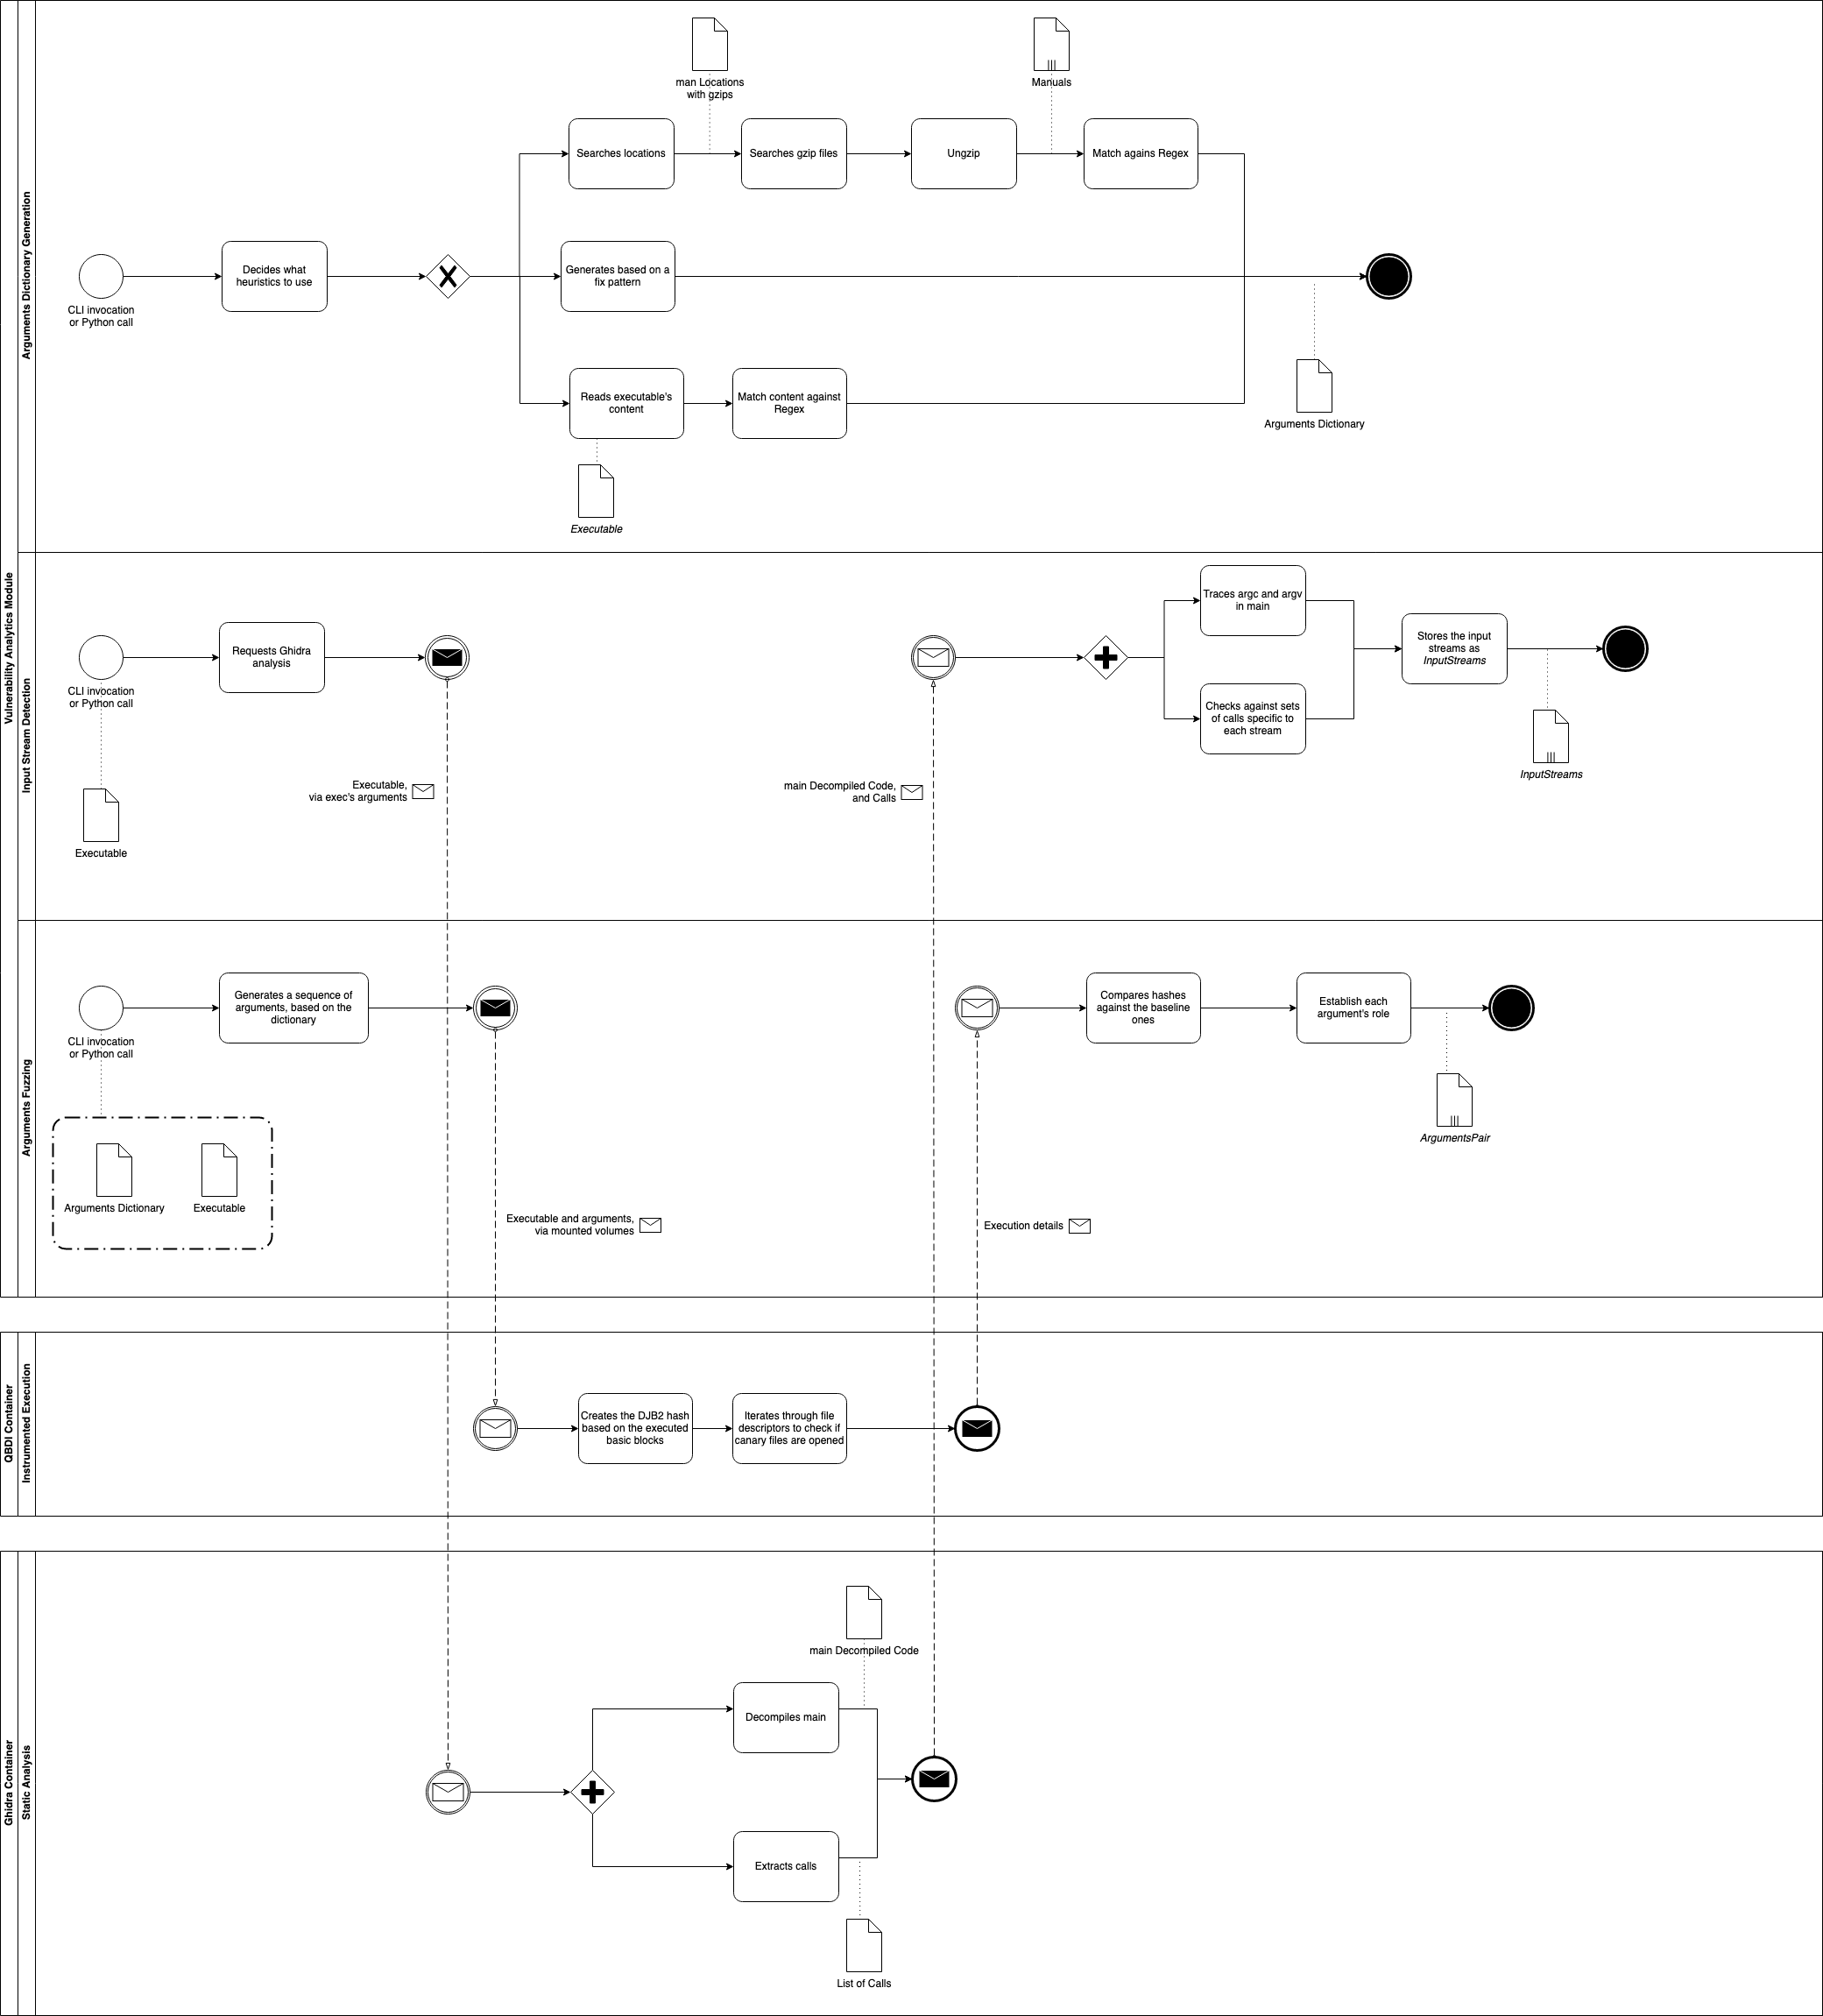
\includegraphics[height=0.85\textheight]{images/surface.png}
    \caption{Architecture of the Attack Surface Approximation Module}
    \label{fig:surface_architecture}
\end{figure}
\vspace*{\fill}
\end{landscape}

\hypertarget{theoretical-considerations}{%
\section{Theoretical
Considerations}\label{theoretical-considerations}}

The paper \cite{security_vuln_likelihood} begins by introducing the concept of front line functions, or
functions adjacent to a source of input. \cite{measuring_attack_surface} expands on this concept by
introducing the concept of direct entry point: a method that includes a
call to one of the specified input methods (for example, \texttt{read}
from \texttt{unistd.h}). Despite the fact that the papers give
theoretical notions that are analogous to the input streams discussed in
this thesis, they do not provide any instrument or approach for
identifying these input entrances in processes. It should also be noted
that the papers approach this topic by studying the source code.

This CRS module, on the other hand, implies creating valid arguments
that can be used in later modules (for example, in vulnerability
identification via fuzzing). Papers such as \cite{cli_fuzzer}\cite{nt_robustness}\cite{power} propose argument
identification, but only with extensive understanding of the
investigated software. To parse, they require a grammar, a
\texttt{getopt} option parsing call, or a man page.

The only implementations identified were in AFL\simplefootnote{https://github.com/google/AFL/tree/master/experimental/argv\_fuzzing}, afl++\simplefootnote{https://github.com/AFLplusplus/AFLplusplus/tree/stable/utils/argv\_fuzzing}, and ManFuzzer\simplefootnote{https://github.com/GroundPound/ManFuzzer}.
The first two have the \texttt{argv\_fuzzing\textquotesingle{}}mode,
which inserts the generated random bytes into the main function's
\texttt{argv}. The third piece of software generates fuzzing sequences
by scanning the man page and the output of programs run with the
\texttt{-h}, \texttt{-H}, and \texttt{-\/-help} options. The downside of
this technique is that it does not take into account the typical format
of an input (e.g.~\texttt{-letter\_or\_word\textgreater{}} or
\texttt{-\/-letter\_or\_word\textgreater{}}). For the latter, there is
an inherent risk that the software lacks a help page or has hidden
arguments (e.g.~experimental ones).

\hypertarget{implementation}{%
\section{Implementation}\label{implementation}}

The purpose of the module in detecting the input streams was divided
into numerous tasks, implying distinct technologies.

\hypertarget{indicators-discovery}{%
\subsection{Indicators Discovery}\label{indicators-discovery}}

The first objective is to statically examine the binary for evidence
(dubbed indications) that a particular input stream is being used. It
should be emphasized that the presence of an indicator is sufficient but
not required. Despite the fact that the program does not call
\texttt{getenv} internally, we cannot guarantee that the environment
variables are not used altogether because the program may employ an
unusual method of parsing its stack to acquire that information.

This analysis aids in the activation of features in the pipeline's
subsequent modules in OpenCRS. For example, if the executable does not
use its command line interface (CLI) arguments, a fuzzer altering (non-existent) arguments
is pointless and will yield no significant findings.

We accomplish this by utilizing the API of a well-known reverse
engineering tool, Ghidra, and confirming the required criteria for
an executable to utilise a specific input stream.

\begin{itemize}
\tightlist
\item
  For arguments: The executable's `main' function is decompiled, and the
  resulting code is processed as an abstract syntax tree. The tree is traversed in order
  to find interactions between the source code of `main' and the
  program's arguments, \texttt{argc} and \texttt{argv}.
\item
  For standard input and files: All function calls are collected into a
  set and repeatedly compared with multiple sets of function names, one
  for each input stream (e.g.~\texttt{("read",\ "fgetc",\ "fread")} for
  \texttt{stdin}). The executable uses an input stream if there is an
  intersection between the two sets.
\end{itemize}

\hypertarget{generating-arguments-dictionaries}{%
\subsection{Generating Arguments
Dictionaries}\label{generating-arguments-dictionaries}}

Before determining whether the binary uses any parameters, a list of
possible arguments should be produced. We used three generation
heuristics:

\begin{itemize}
\tightlist
\item
  \texttt{generation}: Generates parameters while adhering to the
  Regex format \texttt{-{[}a-zA-Z0-9{]}}.
\item
  \texttt{binary\_pattern\_matching}: Looks for bytes sequences in
  binary material that match the Regex
  \texttt{\textbackslash{}s-\{1,2\}{[}a-zA-Z0-9{]}{[}a-zA-Z0-9\_-{]}*}
  (matching, for example, \texttt{-f} and \texttt{-\/-file}).
\item
  \texttt{man\_parsing}: First, it scans the \texttt{man} configuration
  files to determine which folders contain manuals. Finds all gzip files
  in this location, unzips them, and matches their content against
  the same Regex pattern as above. The returned arguments list can
  optionally be reduced to a specified amount of elements based on their
  occurrence.
\end{itemize}

\hypertarget{arguments-fuzzing}{%
\subsection{Arguments Fuzzing}\label{arguments-fuzzing}}

The dynamic approach is better for detecting that an argument (or
combination of arguments) is used by the executable, as the static
approach may result in erroneous results due to superficial inspection
of the control flow graph. By evaluating the program dynamically, on the
other hand, the input causes the program execution to take a different
path, reaching distinct basic blocks (predictable sequences of
instructions, represented as nodes in a control flow graph) and,
subsequently, invoking different system API methods.

The purpose of the subtask is to extract coverage information that can
then be utilized to distinguish between two executions of the same
executable but with different parameters. This information can be
extracted using a variety of dynamic binary analysis approaches,
including:

\begin{itemize}
\tightlist
\item
  Debugging: A debugger can identify the execution flow by establishing
  hardware or software breakpoints on each basic block or system call.
  However, because it is designed for people (programmers, vulnerability
  researchers, etc.), it is not well-suited for automation in which no
  manual interaction is necessary. The performance hit was caused by
  either user-kernel space switches (when invoking the \texttt{ptrace}
  API from the debugger process) or a type of dynamic binary
  instrumentation, which involved rewriting the code with
  debugging-related calls or interrupts.
\item
  Static instrumentation and execution: This method entails translating
  the program into a high-level abstraction language, inserting
  instrumentation code, and compiling it. The newly produced executable
  is then run and can report execution coverage information. This
  strategy, as an alternative to compiler instrumentation, may result in
  unanticipated behavior due to a lack of standardized technology in
  this field of research.
\item
  Dynamic binary instrumentation (DBI): A DBI instrument
  attempts to resolve debugger difficulties. Using Quarkslab's engine,
  QBDI (which is utilized in our implementation), it is possible to
  inject instrumentation code inside the binary at runtime. The
  optimization is that the analysis tool and the analyzed program are
  both performed under the same process, which reduces friction.
\end{itemize}

Following several experiments with the first two methodologies, we found
that the QBDI could be integrated by taking the following steps:

\begin{itemize}
\tightlist
\item
  Convert the executable to a library by removing the Position Independent Execution (PIE) flag (which is
  present in executables) and marking the \texttt{main} function as
  exported with the LIEF Python library.
\item
  \texttt{dlopen} is used to load the executable into program memory.
\item
  Instrument the code with the QBDI C API.
\end{itemize}

It failed because of the QBDI's execution transfer: it deems any calls
to dynamically linked libraries to be non-reentrant and moves the
execution from instrumented to native (with no instrumentation at all).
It returns the instrumentation after the function return.

This limitation prompted us to retry with a different API of QBDI,
\texttt{QBDIPreload}. It is a utility library in which the DBI engine
overwrites and calls all of the callbacks exported by the QBDI API
during runtime. The instrumentation library is loaded into process
memory via the Linux loader's \texttt{LD\_PRELOAD} command. This second
method involved a number of steps:

\begin{itemize}
\item
  Design a callback method to handle basic block calls. To eliminate the
  variations generated by Address Space Layout Randomization, it employs
  an address normalization technique. This relativization of the basic
  block's start address is saved in a list.

\begin{tiny}
\begin{verbatim}
start_address -= segments[parent_segment].start;
abstract_address = (parent_segment << 24) + start_address;
\end{verbatim}
\end{tiny}

\item
  Write a callback function to handle execution transfers. It checks to
  see if \texttt{close} is called on a canary file passed to the
  application as an argument.
\item
  Make a non-cryptographic DJB2 hash over the first 1000 addresses in
  the control flow graph and dump it into a file upon exit.
\end{itemize}

The fuzzing process begins by creating baseline hashes using the
stated coverage extraction mechanism by executing the program with no
arguments and a series of random, 10-character long arguments. Following
that, a series of commands are executed into an Ubuntu-based Docker
container, with a full QBDI setup and communication via mounted Docker
volumes:

\begin{itemize}
\tightlist
\item
  Only a filename as an argument;
\item
  Each argument in the dictionary, one at a time;
\item
  \texttt{-} as an argument; and
\item
  Each argument in the dictionary, one at a time, plus a canary string.
\end{itemize}

Each execution generates a DJB2 hash, which is compared to the baseline
provided. If the hash was not observed until that point, the algorithm
can conclude that the argument resulted in a different execution of the
binary (i.e.~a different sequence of nodes in the control flow graph)
and is therefore registered as a legitimate argument. Aside from that,
each argument has a role that specifies its effects:

\begin{itemize}
\tightlist
\item
  Flag (e.g.~\texttt{-\/-force}): The argument alone generates a unique
  hash.
\item
  File enabler (e.g.~\texttt{-\/-config\ production.yaml}): The program
  is invoked with the current input followed by the name of an OpenCRS
  canary file with the \texttt{.opencrs} extension. On each execution
  transfer, the process's file descriptors are examined to see if the
  canary file is open.
\item
  \texttt{stdin} enabled (e.g.~\texttt{-\/-stdin}): If an execution
  fails due to a timeout, the program is repeated with input from
  \texttt{stdin}. If the hashes produced by these two executions differ,
  the flag is regarded to be enabling \texttt{stdin}-reading
  capabilities and is tagged appropriately.
\item
  String enabler (e.g.~\texttt{-\/-action\ deploy}): The program's
  execution with the arguments alone is compared against one of the
  arguments supplemented with a string. If the first differs from the
  baselines and the latter differs from the first, the argument will be
  assigned this role.
\end{itemize}


\end{document}